\documentclass{article}
\usepackage[margin=1in]{geometry}
\usepackage{amsmath, amssymb, amsthm}
\usepackage{enumitem}
\usepackage{mathtools}
\usepackage{cancel}


% colored links
\usepackage{hyperref}
\hypersetup{
    colorlinks=true,
    linkcolor=blue,
    filecolor=magenta,      
    urlcolor=black!20!BurntOrange,
    }

% Inputting Python code
\usepackage[dvipsnames]{xcolor}
\definecolor{textblue}{rgb}{.2,.2,.7}
\definecolor{textred}{rgb}{0.54,0,0}
\definecolor{textgreen}{rgb}{0,0.43,0}
\usepackage{upquote}
\usepackage{listings}
\lstset{
    language=Python, 
    tabsize=4,
    basicstyle={\ttfamily},
    keywordstyle=\color{textblue},
    commentstyle=\color{textgreen},
    stringstyle=\color{textred},
    frame=none,
    columns=fullflexible,
    keepspaces=true,
    showstringspaces=false,
    xleftmargin=-15mm, % manual adjustment, figure out permanent solution
}

% Drawing figures
\usepackage{tikz}
\usetikzlibrary{calc, shapes.symbols}

% Colored Boxes
\usepackage{tcolorbox}
\tcbuselibrary{skins,hooks}
\usetikzlibrary{shadows}
\usepackage{lipsum}

%Images
\usepackage{graphicx}
    \usepackage{subcaption}
    \usepackage{float}

%Formatting and Spacing
\setitemize[1]{noitemsep, parsep = 5pt, topsep = 5pt}
\setenumerate[1]{label = (\alph*), parsep = 1pt, topsep = 5pt}
\setlength\parindent{0pt}
\linespread{1.1}

%Easy Numbering in case we add or remove questions
\newcounter{counter}
\newcommand{\Exercise}{Exercise \stepcounter{counter}\thecounter}

% \newcommand{\Cov}{\text{Cov}}
% \newcommand{\trace}{\text{trace}}
% \newcommand{\Normal}{\text{Normal}}
% \newcommand{\var}[1]{\operatorname{var}\left(#1\right)}
\newcommand{\E}[1]{\operatorname{E}\left[#1\right]}
\renewcommand{\Pr}[1]{\operatorname{P}\left(#1\right)}

\DeclareMathOperator*{\minimize}{minimize}
\DeclareMathOperator*{\maximize}{maximize}
\DeclareMathOperator*{\argmin}{argmin}
\DeclareMathOperator*{\argmax}{argmax}
\DeclarePairedDelimiter\abs{\lvert}{\rvert}%
\DeclarePairedDelimiter\norm{\lVert}{\rVert}%
\DeclarePairedDelimiterX{\inp}[2]{\langle}{\rangle}{#1, #2}

%Custom Title Fields
\newcommand{\hmwkTitle}{Homework 3 Solutions}
\newcommand{\hmwkDueDate}{Jan.\ 31, 2024}
\newcommand{\hmwkDueTime}{11:59pm EST}
\newcommand{\hmwkClass}{Advanced Algorithms}
\newcommand{\hmwkClassInstructor}{Professor Dana Randall}
\newcommand{\hmwkSection}{Spring 2024}
\newcommand{\hmwkAuthorName}{}

%Headers and Footers
\usepackage{fancyhdr}
\usepackage{extramarks}
\pagestyle{fancy}
\lhead{CS 4540}
\chead{\hmwkClass \ (\hmwkClassInstructor)}
\rhead{\hmwkTitle}
\cfoot{\thepage}
\renewcommand\headrulewidth{0.4pt}
\renewcommand\footrulewidth{0.4pt}

\title{
    \vspace{2in}
    \textbf{\hmwkClass:\ \hmwkTitle}\\
    \normalsize\vspace{0.1in}\small{Due\ on\ \hmwkDueDate\ at \hmwkDueTime}\\
    \vspace{0.1in}\large{\textit{\hmwkClassInstructor\ \hmwkSection}} \\
    \vspace{0.8in}
    \begin{minipage}[t]{0.4\columnwidth}
        {\footnotesize\textbf{As stated in the syllabus, unauthorized use of previous semester course materials is strictly prohibited in this course.
        }}
    \vspace{0.5in}
    \end{minipage}
    \vspace{0.8in}
    \author{\textbf{\hmwkAuthorName}}
    \date{}
}

\begin{document}

\maketitle
\pagebreak

\subsection*{\Exercise}
    \textit{(KT Chapter 13, Exercise 12)}  Consider the following analogue of Karger's
    algorithm for finding minimum $s-t$ cuts.  We will contract edges
    iteratively using the following randomized procedure.  In a given iteration,
    let $s$ and $t$ denote the possibly contracted nodes that contain the
    original nodes $s$ and $t$, respectively.  To make sure that $s$ and $t$ do
    not get contracted, at each iteration we delete any edges connecting $s$ and
    $t$ and select a random edge to contract among the remaining edges.  Give an
    example to show that the probability that this method finds a minimum $s-t$
    cut can be exponentially small.
    
\subsection*{Solution}
    There may be multiple answers. We first consider the small case shown in Figure 1.
    \begin{figure}[H]
      \begin{center}
        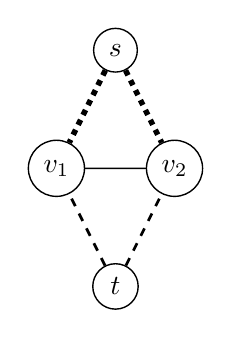
\begin{tikzpicture}[scale=.15]
          \tikzstyle{tvertex}=[circle,edge=black!100]
          \tikzstyle{svertex}=[circle,edge=black!25]
          \tikzstyle{edge}=[draw,line width = .5pt]
          \tikzstyle{sedge}=[draw,line width = 2pt,dotted]
          \tikzstyle{fedge}=[draw,line width = 1pt,dashed]
          \node[tvertex] (s) at (5,20) {$s$};
          \node[tvertex] (t) at (5,0) {$t$};
          \node[svertex] (v11) at (0,10) {$v_1$};
          \node[svertex] (v12) at (10,10) {$v_2$};
          \foreach \v in {v11,v12}{
            \draw[sedge] (s) -- (\v);
            \draw[fedge] (t) -- (\v);
            }
          \foreach \v in {v1}
            \draw[edge] (\v1) -- (\v2);
        \end{tikzpicture}
      \end{center}
      \vspace{-6mm}
      \caption{Simple 4 vertex case}
    \end{figure}
    There are two minimum s-t cuts here, both of size $2$. One cuts both the dotted edges, where the cut puts $s$ on one side, and $v_1, v_2, t$ on the other. The other min s-t cut is the dashed edges, where the cut has $t$ on one side, and $v_1, v_2, s$ on the other side. The other ways to s-t cut the graph have size $3$.

    \vspace{3mm}
    Now we consider the probabilities that we get the min cut: If we contract $v_1$ and $v_2$, then both $v_1$ and $v_2$ will go to one side or another eventually, leaving us with a min-cut. This happens with probability $\frac45$. Now what if we contract another edge, by symmetry say it is $s$ and $v_1$. Now there are two edges between $v_2$ and $\{s,v_1\}$, and one edge between $v_2$ and $t$. Thus, there is a $\frac23$ chance that $v_2$ joins $\{s,v_1\}$, and a $\frac13$ chance that $v_2$ joins $t$. So there is a $\frac{11}{15}$ chance that our cut has size $2$, and a
    $\frac4{15}$ chance that our cut has size $3$. 
    
    \vspace{3mm}
    Let $n$ be even. Now we consider the graph in Figure 2, which has $\frac{n-2}{2}$ copies of the graph from Figure 1.
    \begin{figure}[htbp]
      \begin{center}
        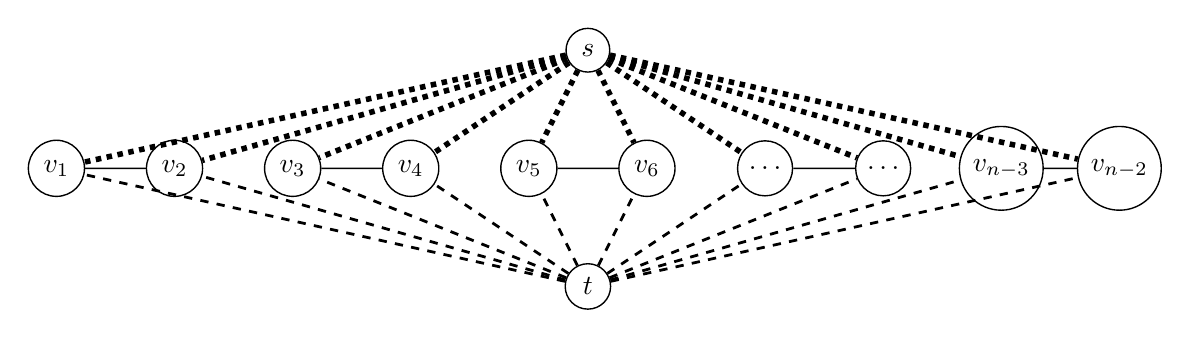
\begin{tikzpicture}[scale=.15]
          \tikzstyle{tvertex}=[circle,edge=black!100]
          \tikzstyle{svertex}=[circle,edge=black!25]
          \tikzstyle{edge}=[draw,line width = .5pt]
          \tikzstyle{sedge}=[draw,line width = 2pt,dotted]
          \tikzstyle{fedge}=[draw,line width = 1pt,dashed]
          \node[tvertex] (s) at (45,20) {$s$};
          \node[tvertex] (t) at (45,0) {$t$};
          \node[svertex] (v11) at (0,10) {$v_1$};
          \node[svertex] (v12) at (10,10) {$v_2$};
          \node[svertex] (v21) at (20,10) {$v_3$};
          \node[svertex] (v22) at (30,10) {$v_4$};
          \node[svertex] (v31) at (40,10) {$v_5$};
          \node[svertex] (v32) at (50,10) {$v_6$};
          \node[svertex] (v41) at (80,10) {$v_{n-3}$};
          \node[svertex] (v42) at (90,10) {$v_{n-2}$};
          \node[svertex] (v51) at (60,10) {$\ldots$};
          \node[svertex] (v52) at (70,10) {$\ldots$};
          \foreach \v in {v1,v2,v3,v4,v5}{
            \draw[sedge] (s) -- (\v1);
            \draw[fedge] (t) -- (\v1);
            \draw[sedge] (s) -- (\v2);
            \draw[fedge] (t) -- (\v2);
            \draw[edge] (\v1) -- (\v2);
            }
        \end{tikzpicture}
      \end{center}
      \vspace{-6mm}
      \caption{n vertex case}
    \end{figure}
    We see that the min s-t cut has size $n-2$, which happens when each pair of nodes $v_{2i-1}, v_{2i}$ either both go to $s$ or $t$. Note that these pairs acts independently of all other pairs. Each pair will be a cut of size 2 with probability $\frac{11}{15}$, and a cut of size 3 with probability $\frac4{15}$, as in the analysis above. So the chance that they all are a cut of size $2$ is $(\frac{11}{15})^{\frac{n-2}{2}}$, which is exponential in $n$, the total number of nodes.


\subsection*{\Exercise}
  Consider the online paging problem in which the access graph $G$ is a line
  on $k+1$ pages. (Recall that in every legal input, every page must be a
  neighbor of the previous one; the first page can be arbitrary.) Recall that
  LRU (least recently used) has competitive ration $1$ on this graph. Show that the competitive
  ratio on $G$ of the FIFO paging algorithm is $k$, the size of the cache.

  Correction: This should be a competitive ratio of $\Omega(k)$.


\subsection*{Solution}
    This question was a bit confusing - some people interpreted it as ``show FIFO is $k$-competitive," while others noticed the comparison to LRU and showed the competitive ratio was $\Omega(k)$, that is, that there was an input on which FIFO/OPT $\geq \alpha k$ for some constant $\alpha$. We accepted both answers, and I'll include both solutions here. On future midterms/finals we'll be more explicit about what you should show.

    \vspace{3mm}
    First, we show that FIFO is k-competitive. That is, we show for any input sequence $\sigma$, the ratio $cost(FIFO)/cost(OPT) \leq k$, where the cost is just the number of faults. For any input sequence of page requests $\sigma$, divide $\sigma$ into consecutive {\it phases} as we did in class, where a phase is a maximal substring containing at most $k$ distinct pages. In each phase, FIFO will fault at most $k$ times - for each of the $k$ pages requested in this phase, there is at most one fault the first time the page is requested. After it is requested once, it will not be thrown out again during this phase because there will always be something that has been in the cache longer that FIFO throws out instead. So, FIFO has at most $k$ faults per phase. We also note that OPT will always have at least one fault per phase. Because the access graph $G$ is a line, phases will alternate with requests for $\{1,...,k\}$ and $\{2,...,k+1\}$, so OPT will keep $\{2,...,k\}$ in the cache at all times and throw out 1 and $k+1$ the next time the other one is requested, which will happen once per phase. Thus, as $cost(FIFO) \leq k$ and $cost(OPT)\geq 1$ for each phase, it follows that $$\frac{cost(FIFO)}{cost(OPT)} \leq k,$$ and so FIFO is $k$-competitive. 

    \vspace{3mm}
    Next, we show that the competitive ratio of $FIFO$ is $\Omega(k)$, that is, there is a constant $\alpha$ such that the competitive ratio of $FIFO$ is at least $\alpha k$. (This is why we added the correction of ``$\Omega(k)$,'' since we can't actually show this for $k$ without $\alpha$.) To show this, we just need to demonstrate one input sequence on which FIFO has at least $\alpha k \cdot OPT$ faults. Consider the request sequence $\sigma = 1,2,\ldots,k,k+1,k,\ldots 2,1,2, \ldots$, that repeatedly requests all items from 1 to k+1 and back to 1. We divide our input sequence into phases that each contain $k$ distinct elements in the standard way. In this case, our phases are alternatingly $1,2,\ldots k$ followed by $k+1,k,\ldots 2$. We will consider our phases in sets of 2.

    \vspace{5mm}
    After the first two phases, we have $2,3,4,\ldots k+1$ in the cache - having arrived in that order. For the next phase, $1$'s arrival will toss out 2, 2's will toss out 3, and so on. Thus we will see $k+1$ faults, for elements $1 \ldots k+1$. Finally $k+1$'s arrival will toss out 1, and we will again have $2 \ldots k+1$ in the cache, having arrived in that order. Now we progress from $k \ldots 2$ without incurring any faults, and we repeat the above argument. Thus, our algorithm will have $k + 1$ faults every two phases.

    \vspace{5mm} OPT will have 2 faults every two phases, as it will only toss out one of 1 and $k+1$ in the cache when you see the other, keeping $2 \ldots k$ in the cache at all times. Thus the competitive ratio is at least $\frac{k+1}{2}$, which is $\Omega(k)$.

\subsection*{\Exercise}
    Consider a paging algorithm that, on a page fault, just throws out a random page from the cache. Prove that the competitive ratio of this algorithm is $\Omega(k)$.

\subsection*{Solution}

% \textbf{Minimum Working Solution}
% Let ALG be the paging algorithm that throws a random page out the cache at each fault. We consider the pages as numbers  $1 \ldots k+1$. We'll show there's a request sequence $\sigma$ on which ALG throws, in expectation, a factor of $k$ more faults than OPT, the optimal paging algorithm for that sequence of requests.

% Consider the sequence that starts with $k+1$ and then repeats $1,2,...,k$ some large number of times. We'll assume both ALG and OPT start with empty caches, and so they first populate their cache with $k+1, 1,2,3,..., k-1$. When page $k$ is requested next, OPT will fault and throw out page $k+1$, but then will not fault for the remainder of the input sequence. thus OPT has one total fault. 

% However, ALG will just throw out a random page $i$ when page $k$ is requested. If $i \neq k+1$, then the next time page $i$ is requested, ALG will fault again and throw out some other random page $j$. This will continue until ALG randomly throws out page $k+1$, after which it will not have any more faults. At each fault, the probability that $k+1$ is thrown out is $1/k$. Let $X$ be a random variable denoting the number of faults until $k+1$ is thrown out. We know $X$ is a geometric random variable with parameter $1/k$; the random variable measures the number of coin tosses needed to get heads, if heads occurs with probability $1/k$. A Geometric($1/k$) random variable has expectation $k$, and so we have $k$ expected faults, $\E[X] = k$. It follows then that on input $\sigma$ as described above, $$\frac{\E[cost(ALG)]}{cost(OPT)} = \frac{k}{1} = \Omega(k).$$


\textbf{Full Solution}
    Let ALG be the paging algorithm that throws a random page out of the cache at each fault. We consider the pages as numbers $1 \ldots k+1$. 
    We'll show there's a request sequence $\sigma$ on which ALG throws, in expectation, a factor of $k$ more faults than OPT, the optimal paging algorithm for that sequence of requests. 

    \vspace{3mm}s
    Consider the request sequence that has $1,....,k$ repeated $m$ times (we'll specify $m$ later, for now just think of it as large), followed by a request for $k+1$; call this one {\i  t round}. The request sequence $\sigma$ then contains an arbitrary number of rounds. Note that this isn't quite the same as a {\it phase} as we defined in class, but it captures the same ideas and will be much easier to work with. 

    \vspace{3mm}
    We assume that the cache, for both OPT and ALG, has page $k+1$ in it to start, and does not have some page $i$. The first time $i$ is requested, OPT will fault and will throw out $k+1$; when page $k+1$ is requested as the last page in the round, OPT will fault again and throw out some other page. Thus, OPT has two faults per round. 

    \vspace{3mm}
    The first time $i$ is requested in the round, ALG will fault and randomly throw out some other page $j$. ALG will then fault again and again until the random page it chooses to throw out is $k+1$, at which point it won't fault again the rest of the round until $k+1$ is requested as the last page of the round. At each fault the probability that $k+1$ will be thrown out is $1/k$, independently of any previous attempts to throw out $k+1$. Let $X$ be a random variable denoting  the number of faults until $k+1$ is thrown out; for now, we assume $m$ is arbitrarily large, and we will come back and bound it later. We know $X$ is a geometric random variable with parameter $1/k$; the random variable measures the number of coin tosses needed to get heads, if heads occurs with probability 1/k. $X \sim \text{Geo}(1/k)$ has expectation $k$, and so we have $k$ expected faults. 

    \vspace{3mm}
    However, as $\sigma$ must be a finite string, and it's possible that the round might end without throwing $k+1$ out of the cache. 
    So our random variable should actually be the expected number of tosses needed to get heads, but we are cut off after some number of attempts $Y$. Then we can think of the total number of faults of random algorithm ALG on one round of request sequence $\sigma$, which we'll denote $ALG(\sigma)$, as $\min(X,Y)$, where $X$ is the geometric random variable above, $Y$ is our cutoff. If $k+1$ is thrown out during the round there will be one additional fault for the last page request of the round, but since all we're trying to do is lower bound the number of faults we'll disregard this one to make the analysis simpler. 

    \vspace{3mm}
    Unfortunately, $Y$ is a complicated random variable that depends on the actual outcomes of the tosses. However, we know that if $k+1$ is still in our cache, we will have at least 1 fault per round, thus $Y \geq m$. So, $$ALG(\sigma) \geq \min(X,Y) \geq \min(X,m).$$ This we can analyze: let $p = 1/k$, and let $q = 1 - 1/k$. Then $$\Pr{ \min(X,m)= k} =  \left\{ \begin{array}{cc} pq^{k-1} & k < m \\ q^{k} & k=m \\ \end{array} \right. $$ It then follows that $$\E{ ALG(\sigma)} \geq \E{ \min(X,m)} = \sum_{i=1}^{m} i \Pr{\min(X,m) = i}  = \sum_{i=1}^{m-1} ipq^{i-1} + mq^{m-1} = \frac{1 - q^m}{p} = k(1 - q^m).$$ If we set $m = k$, then $q^m = (1 - 1/k)^k \leq e^{-1}$. Thus $\E{ ALG(\sigma)} \geq (1 - e^{-1})k = \Omega(k)$. To bound the competitive ratio, we see that, if we similarly let $OPT(\sigma)$ denote the number of faults OPT has on request sequence $\sigma$, $$ \frac{\E{ ALG(\sigma)}}{OPT(\sigma)} \geq \frac{(1 - e^{-1})k}{2} = \Omega(k).$$

\subsection*{\Exercise}
    Suppose you are standing next to a long fence that extends as far as you can see in either direction. You want to cross the fence and you know that somewhere it has a hole in it, but you don't know whether the hole is to your left or to your right, or how far away the hole is. We can model the problem as follows: you are initially located at the origin on the real line. The hole is at some unknown positive or negative integer coordinate h (why can we assume h is an integer?). You can move left or right at cost equal to the distance moved, and the game continues until you reach h. We will consider the goal of minimizing the competitive ratio: i.e., the ratio of the distance traveled and $\abs{h}$.
    \begin{enumerate}
        \item Give a deterministic strategy with competitive ratio 9. (Hint: Consider walking 1 unit to the right, 2 units to the left, 4 to the right, 8 to the left, etc.)
        \item Describe and analyze a randomized algorithm whose competitive ratio is at most 7. (I.e. Show that for any h, the expected cost of the algorithm is at most $7\abs{h}$).
        \item  Give a randomized algorithm that is better than 7 competitive. It does not have to be optimal, any $(7-\varepsilon)$-competitive algorithm will suffice.
    \end{enumerate}

\subsection*{Solution}
  \begin{enumerate}
  \item The hint says to consider the deterministic strategy where we walk 1 unit to the right, 2 to the left, 4 to the right, 8 to the left, etc. To make the analysis simpler, we assume we move back to the origin after each of these moves. That is, we move to $1, -2, 4, -8, 16, ....$; we call these values the {\it turning points}. Our position after the $ith$ step is then $(-2)^i$ (if we start by calling our move to 1 the 0th step). 
      
      First, consider the case where $h$ is positive. Let $h = h^* + k$, $k > 0$, where $h^* = 2^i$ is the largest turning point less than $h$; it must be that $i$ is even, $i = 2j$ for some $j$. 
      
      To reach $h$, OPT simply walks to location $h$, for a cost of $h = 2^i + k$. 
      
      To reach $h$, ALG walks to each of the locations $1,-2,.... -2^{i-1}, 2^i, -2^{i+1}$ and back to the origin, before walking right and reaching $h$. Thus, the total distance covered by ALG is
      $$ 2 ( 1 + 2 + 4 + ... + 2^{i+1}) + 2^i + k = 2 ( 2^{i+2} - 1) + 2^i + k) = 8 \cdot 2^i -2 + 2^i + k = 9\cdot 2^i+k-2 $$
    Now, suppose $h$ is negative. Let $h = h^* - k$, $k > 0$, where $h^* = -2^i$ is the smallest turning point more than $h$; it must be that $i$ is odd, $i = 2j + 1$ for some $j$. 
    
    To reach $h$, OPT simply walks to location $h$, for a cost of $h = 2^i + k$. 
    
    To reach $h$, ALG walks to each of the locations $1,-2,.... ,+2^{i-1}, -2^i, +2^{i+1}$ and back to the origin, before walking right and reaching $h$. Thus, the total distance covered by ALG is
    $$ 2 ( 1 + 2 + 4 + ... + 2^{i+1}) + 2^i + k = 9 \cdot 2^i +k-2  $$
            
    In either case, we see that $$\frac{cost(ALG)}{cost(OPT)} = \frac{9 \cdot 2^i +k-2}{2^i + k} \leq \frac{9 \cdot 2^i +9k}{2^i + k} = 9$$
  
    % \item The hint says to consider the deterministic strategy where we walk
    %   1 unit to the right, 2 to the left, 4 to the right, 8 to the left, etc.
    %   We call each alternation a $turn$.
    %   After moves to the right on odd turns 2i+1, our positions are +1, +3, +11,
    %   +43, \ldots, $1 + 2\frac{4^i-1}{3}$. On even moves $2i$, our final
    %   positions are -1, -5, -21, \ldots $-\frac{4^i - 1}{3}$. We call these
    %   $\emph{turning points}$.

    %   For now, consider the case where $h$ is positive.
    %   Let $h = h^* + k$, where $h^*$ is the nearest of the above turning
    %   points less than $h$, and $k>1$ is the extra distance beyond the
    %   turning point to reach $h$.

    %   For positive $h$, then $h = 1 + k + 2\frac{4^i -1}{3}$. To get here, we
    %   take $1 + 2 + \ldots 2^{2i} + 2^{2i+1} + (2^{2i+1} + k)$ total steps.
    %   The parenthesized amount is the amount taken on the last step -
    %   backtracking $2^{2i+1}$ and then taking k extra steps. This simplifies
    %   to exactly $3 \cdot 2^{2i + 1} + k-1$ steps.
    %   Thus, $$\frac{ALG}{OPT} = \frac{3 \cdot 2^{2i+1} + k - 1}
    %   {1 + k + 2\frac{4^i -1}{3}}
    %   = \frac{9 \cdot 2 \cdot 4^i + 3k-3}{2 \cdot 4^i + 3k + 7/3} \leq 
    %    \frac{9 \cdot 2 \cdot 4^i + 9k+9}{2 \cdot4^i + k + 1} = 9.$$

    %   If $h$ is negative, the analysis is very similar. Let $h = h^* - k$, where $h^*$ is the nearest of the turning points above that is greater than $h$, and $k$ is the extra distance past that turning point we have to go to reach $h$. 
    %   Since $h$ is negative in this case, $h = -\frac{4^i - 1}{3} - k$. To get here we take $1 + 2 + 4 + ... + 2^{2i} + \left(2^{2i} + k \right)$ total steps. The number of total steps then simplifies to $3\cdot 2^{2i} + k - 1$.Thus, 
    %   $$\frac{ALG}{OPT} = \frac{3 \cdot 2^{2i} + k - 1}
    %   {\frac{4^i - 1}{3} + k}
    %   = \frac{9 \cdot 4^i + 3k-3}{4^i + 3k - 1} \leq 
    %    \frac{9 \cdot 4^i + 27k}{4^i + 3k} = 9.$$
      
    %   Thus, this deterministic algorithm has competitive ratio 9. 
      
      
      \item ALGORITHM: We flip an unbiased coin at the very beginning to decide if we start going left or
      right, then perform the above alternating strategy.
      
     
      
      This time, without loss of generality, assume $h$ is positive. The turning points are the same as above, but with probability 1/2 their signs are reversed.  Pick $i$ such that $2^i$ is the largest power of 2 strictly less than $h$, and let $h = 2^i + k$, $k > 0$.  Note that as above, $cost(OPT) = h = 2^i + k$.  With probability 1/2, value $2^i$ is a turning point, and with the remaining probability 1/2, value $-2^i$ is a turning point. We'll calculate the cost in each of these cases and average our answers to get the expected cost of ALG. 
      
      First, suppose $2^i$ is a turning point. ALG will travel to $2^i$, then to $-2^{i+1}$, and then return and reach $h$. The cost of this is 
      $$2(1 + 2 + ... + 2^i + 2^{i+1}) + 2^i +k  = 2(2^{k+2}-1) + 2^i + k = 9 \cdot 2^i + k-2.$$

      Now suppose $-2^i$ is a turning point. ALG will travel to $2^{i-1}$, $-2^i$, and then will try to travel to $2^{i+1}$ and will find $h$ along the way. The total cost of this is  
      $$2(1 + 2 + ... + 2^{i-1} + 2^{i}) + 2^i +k  = 2(2^{k+1}-1) + 2^i + k = 5 \cdot 2^i + k-2.$$   
      
Averaging, we see that the expected cost of ALG is 
$$ \E{cost(ALG)} = \frac12 \left(  9 \cdot 2^i + k -2\right) + \frac12\left(5 \cdot 2^i + k-2\right) = 7 \cdot 2^i + k-2$$

Comparing this to the cost of OPT, we find that ALG is 7-competitive: 
$$\frac{\E{cost(ALG)}}{cost(OPT)} = \frac{7 \cdot 2^i + k-2}{  2^i + k} \leq \frac{7 \cdot 2^i +7k}{  2^i + k}  = 7.$$
      
      
      \iffalse
      
    \item
      \textbf{Algorithm.} We flip an unbiased coin at the very beginning to decide if we start going left or
      right, then perform the above alternating strategy.

      \vspace{2mm}
      This time, without loss of generality, assume $h$ is positive.
      We call the turning points if we take the left route the left turning
      points, and similarly define right turning points.  Now, the turning
      points are the same as above, but their signs may be reversed depending
      on the direction our algorithm takes.

        \vspace{2mm}
      We first note that the turning points alternate:
      $\frac{4^i - 1}{3} \leq 1 + 2\frac{4^i -1}{3} \leq \frac{4^{i+1}}{3}
      \ldots$.

    \vspace{2mm}
      First, suppose $1 + 2\frac{4^i -1}{3} < h \leq \frac{4^{i+1} -1}{3}$ for some $i$.
      As before, let $h - (1 + 2\frac{4^i -1}{3}) = k$. If we take the left route, we travel a total of
      $1 + 2 + \ldots 2^{2i+1} + 2^{2i+1} + k = 3 \cdot 2^2i _ k -1$ steps as above.

    \vspace{2mm}
      If we take the right route, then the last turning point was
      $\frac{4^{i-1}}{3}$. Now, we travel a total of
      $$1 + 2 + \ldots 2^{2i-1} + 2^{2i} + \left(2^{2i+1}-\left(\frac{4^{i+1} -1}{3} -
      \left(1 + 2\frac{4^i - 1}{3}\right)\right) + k\right)$$
      $$ = 2 \cdot 2^{2i+1} - 1  - \left( \frac{2 \cdot 4^i+ 1}{3}\right) +  1 + k$$
      $$ = 4 \cdot 4^i -  \left( \frac{2 \cdot 4^i+ 1}{3}\right) + k$$ 
      $$ = \frac{10}{3} 4^i - \frac{1}{3} + k$$


      We are equally likely to take either route, so our expected travel
      distance is, with algebraic simplification,
      $$\frac{1}{2}\left\{ (3 \cdot 2^{2i + 1} + k-1)
      + \left(\frac{10}{3} 4^i - \frac{1}{3} + k\right)
      %(2 \cdot 2^{2i+1} - 1 - 2\frac{4^i-1}{3} + k
      \right\}
      = \frac12 \bracksfit{\frac{28}{3}\cdot 4^{i} + 2k - \frac43} 
      = \frac{14}{3} 4^i + k - \frac23 $$

      Then the ratio ALG/OPT is:
      $ \frac{ \frac{14}{3} 4^i + k -\frac23}{ 1 + 2\frac{4^i -1}{3} + k}
      = \frac{7 * 4^i +3k/2 - 1}{4^i + 3k/2 + 1/2} \leq 7 $ as desired.
      
      It remains to consider the other case, $\frac{4^{i} -1}{3} < h \leq 1 + 2\frac{4^i -1}{3} $ for some $i$. Pick $k$ such that $h = \frac{4^{i} -1}{3} + k$. 
      
       If we take the right route, as above we travel  $1 + 2 + 4 + ... + 2^{2i} + \left(2^{2i} + k \right) = 3\cdot 2^{2i} + k - 1$ total steps. 
       
       If we take the left route, the total steps we travel is 
      \begin{align*}
         1 + 2 + \ldots 2^{2i-1} +& \left(2^{2i} - \left(1 + 2\frac{4^i-1}{3} - \frac{4^i-1}{3}\right)+ k\right) \\
         &= 2 \cdot 2^{2i} - 1 -1 - 2\frac{4^i-1}{3} + \frac{4^i-1}{3}+ k \\
         &=  2 \cdot 2^{2i}  -  \frac{4^i-1}{3}+ k - 2 \\
         &= \frac53 4^i+ k - \frac53
    \end{align*}
    
    We are equally likely to pick either route, so our expected travel distance is 
    $$ \frac12\left\{ \left(3\cdot 2^{2i} + k - 1\right) + \left( \frac53 4^i+ k - \frac53 \right) \right\}
    = \frac12\left\{ \frac{14}{3} 4^i + 2k - \frac83\right\}
    = \frac73 4^i + k - \frac43 . $$
    
    Then, the ratio ALG/OPT is: 
    
  $$  \frac{\frac73 4^i + k - \frac43 }{\frac{4^{i} -1}{3} + k} 
  = \frac{ 7 \cdot 4^i + 3k - 4}{4^i +3k - 1} \leq 7$$
    
    Thus, this randomized algorithm has a competitive ratio of 7. 
    
  
  \fi


        
 \item 
      We can achieve a better that 7 ratio by essentially doing the above
      strategy, increasing the amount we jump by a ratio other than 2. We'll
      use 2.5 for the below example. 

      \textbf{Algorithm: } Choose the left route with probability 1/2 and the right route with probability 1/2. We jump between positions
      $1,-2.5,{2.5^2},- 2.5^3 ,\ldots , 2.5^i $ if we choose the left route, and the negatives
      of these if we choose the right route. 

      Without loss of generality, say $h$ is positive, and say $2.5^i < h \leq 2.5^{i+1}$. As before, let
      $h - 2.5^i = k$.

      One of the routes will turn at $2.5^i$ and back at $-2.5^{i+1}$. 
      This will have the following total cost, which we simplify using the geometric sum formula:
      \begin{align*}
      2 (1 + 2.5 + &2.5^2 + ... + 2.5^i + 2.5^{i+1})  + 2.5^i + k\\
      & = 2 \cdot\frac{2.5^{i+2} -1}{2.5-1} + 2.5^i + k \\& = \frac{4}{3} (2.5^{i+2} - 1) + 2.5^i + k
\end{align*}
      The other route will have turned at $2.5^{i-1}$ and back at $-2.5^i$. This has total cost
          \begin{align*}
      2 (1 + 2.5 + &2.5^2 + ... + 2.5^i)  + 2.5^i + k\\
      & = 2 \cdot\frac{2.5^{i+1} -1}{2.5-1} + 2.5^i + k \\& = \frac{4}{3} (2.5^{i+1} - 1) + 2.5^i + k
\end{align*}        
       Our expected distance is then, with some algebraic simplification, is
      \begin{align*}
      \E{cost(ALG)} =  \frac12&\left\{ \frac{4}{3} (2.5^{i+2} - 1) + 2.5^i + k + \frac{4}{3} (2.5^{i+1} - 1) + 2.5^i + k \right\} \\
      &= \frac23(2.5^2 + 2.5) 2.5^i  - \frac23 + 2.5^i +k\\
       &= \left(\frac{41}{6}\right) 2.5^i + k - \frac23
       \end{align*}
      
      Thus, the competitive ratio is $$\frac{\E{ALG(h)}}{OPT(h)} = \frac{\frac{41}{6}2.5^i + k - \frac23}{2.5^i + k}
    \leq \frac{41}{6} < 6.83334 < 7$$.
  \end{enumerate}




\end{document}
